\documentclass[../../../include/open-logic-section]{subfiles}

\begin{document}

\olfileid{sth}{ordinals}{idea}	
\olsection{الفكرة العامة للعدد الترتيبي}

انظر في الأعداد الطبيعية بترتيبها المعتاد:
\begin{center}
	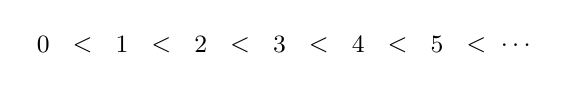
\begin{tikzpicture}
	\foreach \x/\xtext in {0, 1, 2, 3, 4, 5}
	{
		\node (\x a) at (\x, 1) {\small{$\x$}};
		\node (\x a) at (\x.5, 1) {\small{$<$}};
	}
	\node (ldots) at (6, 1) {\small{$\ldots$}};
	\end{tikzpicture}
\end{center}
نسمي هذا، في الاصطلاح الفني، متتالية من النمط~$\omega$. وهذا الترتيب
العام نفسه ينعكس بالفعل في بنائنا الأولي لمراحل هرم المجموعات. لكن
افترض الآن أننا نقلنا~$0$ إلى نهاية هذه المتتالية، بحيث يأتي بعد جميع
الأعداد الأخرى:
\begin{center}
	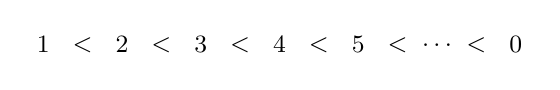
\begin{tikzpicture}
	\foreach \x/\xtext in {1, 2, 3, 4, 5}
	{
		\node (\x a) at (\x, 1) {\small{$\x$}};
		\node (\x a) at (\x.5, 1) {\small{$<$}};
	}
	\node (ldots) at (6, 1) {\small{$\ldots$}};
	\node (bea) at (6.5, 1) {\small{$<$}};
	\node (noa) at (7, 1) {\small{$0$}};
	\end{tikzpicture}
\end{center}
لدينا هنا الكيانات نفسها، لكنها مرتبة ترتيبًا مختلفًا اختلافًا
جوهريًا: لم يكن لترتيبنا الأول عنصر أخير، أما ترتيبنا الجديد فله عنصر
أخير. والواقع أن ترتيبنا الجديد يتألف من متتالية من النمط~$\omega$
من الكيانات ($1, 2, 3, 4, 5, \ldots$)، يتلوها كيان آخر. ومن ثم فهو
متتالية من النمط~$\omega+1$.

ونستطيع توليد أنماط أخرى أكثر من الترتيب باستعمال هذه الكيانات وحدها.
فانظر مثلًا في جميع الأعداد الزوجية (بترتيبها الطبيعي)، تتلوها جميع
الأعداد الفردية (بترتيبها الطبيعي):
\begin{center}
	\begin{tikzpicture}
	\node(a1) at (1,1) {\small{$0$}};
	\node(a2) at (1.5,1) {\small{$<$}};
	\node(a3) at (2,1) {\small{$2$}};
	\node(a4) at (2.5,1) {\small{$<$}};
	\node(a5) at (3,1) {\small{$4$}};
	\node(a6) at (3.5,1) {\small{$<$}};
	\node(dots) at (4,1) {\small{$\ldots$}};
	\node(aaoe) at (4.5,1) {\small{$<$}};
	\node(b1) at (5,1) {\small{$1$}};
	\node(b2) at (5.5,1) {\small{$<$}};
	\node(b3) at (6,1) {\small{$3$}};
	\node(b4) at (6.5,1) {\small{$<$}};
	\node(b5) at (7,1) {\small{$\ldots$}};
	\end{tikzpicture}
\end{center}
هذه متتالية من النمط~$\omega$ تتلوها متتالية أخرى من النمط~$\omega$؛
أي متتالية من النمط~$\omega+\omega$.

وبوسعنا بالطبع مواصلة ذلك. لكن ما نريده هو طريقة عامة لفهم هذا الحديث
عن \emph{الترتيبات}.

\end{document}
